\documentclass[10pt]{article}
% ! ========================
% ! # MARK: Template Control
% ! ========================

% Defines the template variant. Can be 'essay' (default) or 'paper'.
% This command must come before the document class definition in the main file.
\providecommand{\templatevariant}{essay}


% ! =======================
% ! # MARK: Package Loading
% ! =======================

% Common Packages
\usepackage[T1]{fontenc} % Font encoding
\usepackage{tgtermes} % TeX Gyre Termes font (Times clone)
\usepackage{geometry} % Page layout control
\usepackage{setspace} % Line spacing control
\usepackage{graphicx} % Enhanced graphics
\usepackage{xcolor} % Color definitions
\usepackage{colortbl} % Color in tables
\usepackage{hhline} % Double horizontal lines in tables
\usepackage{makecell} % Thicker lines in tables
\usepackage{tabularx, booktabs} % Advanced table layouts
\usepackage{enumitem} % Custom list environments
\usepackage{amsmath} % Advanced math environments
\usepackage{amssymb} % Math symbols
\usepackage{siunitx} % SI units package
\usepackage{listings} % Code listings
\usepackage{natbib} % Bibliography and citations
\usepackage{authblk} % Author and affiliation blocks
\usepackage{tocloft} % ToC, LoF, LoT styling
\usepackage[nottoc]{tocbibind} % Add Bib, Index, etc., to ToC
\usepackage{microtype} % Improved typography (justification, spacing)
\usepackage{url} % URL formatting
\usepackage[breaklinks,linktocpage]{hyperref} % Hyperlinks (must be loaded late)

% Variant-Specific Packages
% Define variant names for comparison
\def\papervariant{paper}
\def\essayvariant{essay}

% Load packages only required for the 'paper' template
\ifx\templatevariant\papervariant
  \usepackage{multicol}     % For multi-column layout
  \usepackage{dblfloatfix}  % Fixes for double-column floats
\fi


% ! ==============================
% ! # MARK: Page Layout & Geometry
% ! ==============================

\ifx\templatevariant\papervariant
  % Paper Template Layout (Two-Column)
  \geometry{
    left=3cm,
    right=3cm,
    top=2.5cm,
    bottom=3cm
  }
  % Settings for two-column layout
  \setlength{\columnseprule}{0pt} % No vertical rule between columns
  \setlength{\columnsep}{0.7cm}   % Space between columns
\else
  % Essay Template Layout (Single-Column, Default)
  \geometry{
    left=4cm,
    right=4cm,
    top=3cm,
    bottom=3.5cm
  }
\fi


% ! ==========================
% ! # MARK: Typography & Fonts
% ! ==========================

% Page Numbering
\renewcommand{\thepage}{\footnotesize\arabic{page}}

% List Spacing
\setlist[itemize]{noitemsep, topsep=7pt, partopsep=0pt, leftmargin=*, label=\textendash}


% ! ================================
% ! # MARK: Floats, Figures & Tables
% ! ================================

% Float Placement Parameters
\renewcommand{\topfraction}{0.9}
\renewcommand{\bottomfraction}{0.8}
\renewcommand{\textfraction}{0.1}
\renewcommand{\floatpagefraction}{0.8}
% Additional float settings for two-column paper template
\ifx\templatevariant\papervariant
  \renewcommand{\dbltopfraction}{0.9}
  \renewcommand{\dblfloatpagefraction}{0.8}
\fi

% Caption Styling
\usepackage[font=footnotesize,skip=7pt,labelfont=bf]{caption}
\captionsetup{justification=raggedright} % Left-align all captions
\newcommand{\floatcaption}[2]{\caption[#1.]{#1~#2.}} % Custom caption command


% ! ================================
% ! # MARK: Bibliography & Citations
% ! ================================

\renewcommand{\bibname}{References} % Change bibliography title
\setlength\bibindent{0pt}           % No indentation for bibliography entries

% Adjust layout and font size in the bibliography environment
\let\oldthebibliography=\thebibliography
\let\endoldthebibliography=\endthebibliography
\renewenvironment{thebibliography}[1]{%
  \begin{oldthebibliography}{#1}%
    \raggedright%
    \footnotesize%
    \setlength{\itemsep}{3pt}%
    \setlength{\parsep}{0pt}%
    \setlength{\parskip}{0pt}%
    }{%
  \end{oldthebibliography}%
}


% ! =====================
% ! # MARK: Code Listings
% ! =====================

% Custom Colors for Code
\definecolor{codegreen}{rgb}{0,0.5,0}
\definecolor{codegray}{rgb}{0.4,0.4,0.4}
\definecolor{codepurple}{rgb}{0.58,0,0.82}
\definecolor{backcolour}{rgb}{0.96,0.96,0.96}
\definecolor{lightgray}{gray}{0.8}

% Language Definition (Example: JavaScript)
\lstdefinelanguage{JavaScript}{
  keywords={break, case, catch, continue, debugger, default, delete, do, else, finally, for, function, if, in, instanceof, new, return, switch, this, throw, try, typeof, var, void, while, with},
  morecomment=[l]{//},
  morecomment=[s]{/*}{*/},
  morestring=[b]',
  morestring=[b]",
  sensitive=true
}

% Listing Style Definition
\lstdefinestyle{mystyle}{
  backgroundcolor=\color{backcolour},
  commentstyle=\color{codegreen},
  keywordstyle=\color{purple},
  numberstyle=\tiny\color{codegray},
  stringstyle=\color{codepurple},
  basicstyle=\ttfamily\footnotesize,
  breakatwhitespace=false,
  breaklines=true,
  captionpos=b,
  frame=tb,
  framerule=0pt,
  framextopmargin=6pt,
  framexbottommargin=6pt,
  keepspaces=true,
  numbers=left,
  numbersep=5pt,
  showspaces=false,
  showstringspaces=false,
  showtabs=false,
  tabsize=2
}
\lstset{style=mystyle} % Apply the defined style globally


% ! ===================================
% ! # MARK: Document Structure & Titles
% ! ===================================

% Table of Contents (ToC)
\renewcommand{\contentsname}{Table of Contents}
\renewcommand\cftsecafterpnum{\vskip8pt}              % Vertical space after section numbers
\renewcommand{\cftsecleader}{\cftdotfill{\cftdotsep}} % Dotted leaders for sections

% List of Listings (LoL)
\renewcommand{\lstlistlistingname}{List of \lstlistingname s}


% ! ==========================
% ! # MARK: Hyperlinks & URLs
% ! ==========================

\hypersetup{
  colorlinks = true,
  urlcolor   = blue,
  linkcolor  = blue,
  citecolor  = blue,
  breaklinks = true
}
% URL Line Breaking
\PassOptionsToPackage{hyphens}{url}
\urlstyle{same}
\def\Urlmuskip{0mu plus 1mu}
\def\UrlBreaks{\do\/\do-}
\def\UrlBigBreaks{\do\/\do-\do:\do.}


% ! =======================
% ! # MARK: Draft Watermark
% ! =======================

% Uncomment the following lines to add a "DRAFT" watermark on every page.
% \usepackage{background}
% \backgroundsetup{contents=DRAFT, opacity=0.25, color=gray}
% Line Spacing
% \doublespacing % Uncomment for review drafts


\begin{document}
% Changing the initial page numbering to uppercase Roman
\pagenumbering{roman}
% Resetting the page counter to 1
\counterwithin{lstlisting}{section}
\counterwithin{figure}{section}
\counterwithin{table}{section}
% Sets the distance between the bottom and the footer
\setlength{\footskip}{65pt}

% ! ===============================
% ! Start of the title page content
% ! ===============================

\title{\textbf{WebGPU vs Pixel Streaming:} \\ A View From Afar}
\author[1]{Daniel Burger}
\affil[1]{\textbf{Middlesex University London\thanks{In collaboration with SAE Institute Zürich.}}}
\affil[ ]{\href{mailto:public@danielburger.online}{public@danielburger.online}}
\date{\textit{7. February 2021}}
\maketitle
% Resetting the page style for the first page
\thispagestyle{empty}

% The sloppypar environment adjusts the spaces between words such that each line fits into the text width
\begin{sloppypar}
  \begin{abstract}
    Two completely new technologies to develop modern graphics-focused software are on the rise. WebGPU is the successor to WebGL and offers remarkable performance improvements. However, pixel streaming goes in a completely different direction and is actively used by the gaming industry.

    In this article, we go into the near future and look at a hypothetical 3D application’s top-level architecture and argue the pros and cons of WebGPU vs pixel streaming from a developer’s perspective.
  \end{abstract}

  \pagebreak
  % Changing the page numbering back to uppercase Roman
  \pagenumbering{Roman}
  \tableofcontents
  \pagebreak
  \listoffigures
  \pagebreak
  \listoftables
  \pagebreak
  \addcontentsline{toc}{section}{\lstlistlistingname} % Add to the TOC
  \lstlistoflistings
  \pagebreak
  % Changing the page numbering back to Arabic
  \pagenumbering{arabic}

  % ! ====================================
  % ! Start of the actual document content
  % ! ====================================

  \section{Introduction}
  \label{sec:introduction}

  A company that wants to develop software asks itself at some point in the development process which technologies they should use. The investment in terms of future viability is a point to consider; e.g. if company XYZ writes an app with Perl, they will probably have difficulties finding new developers in 20 years who can continue developing with this technology (The HFT Guy, 2019).

  The following passages will argue about two technologies that raise important questions for developing 3D applications in the next few years: In which direction should companies/developers invest? What are the advantages and disadvantages and above all: what are these technologies?

  \begin{figure}[ht]
    \centering
    \frame{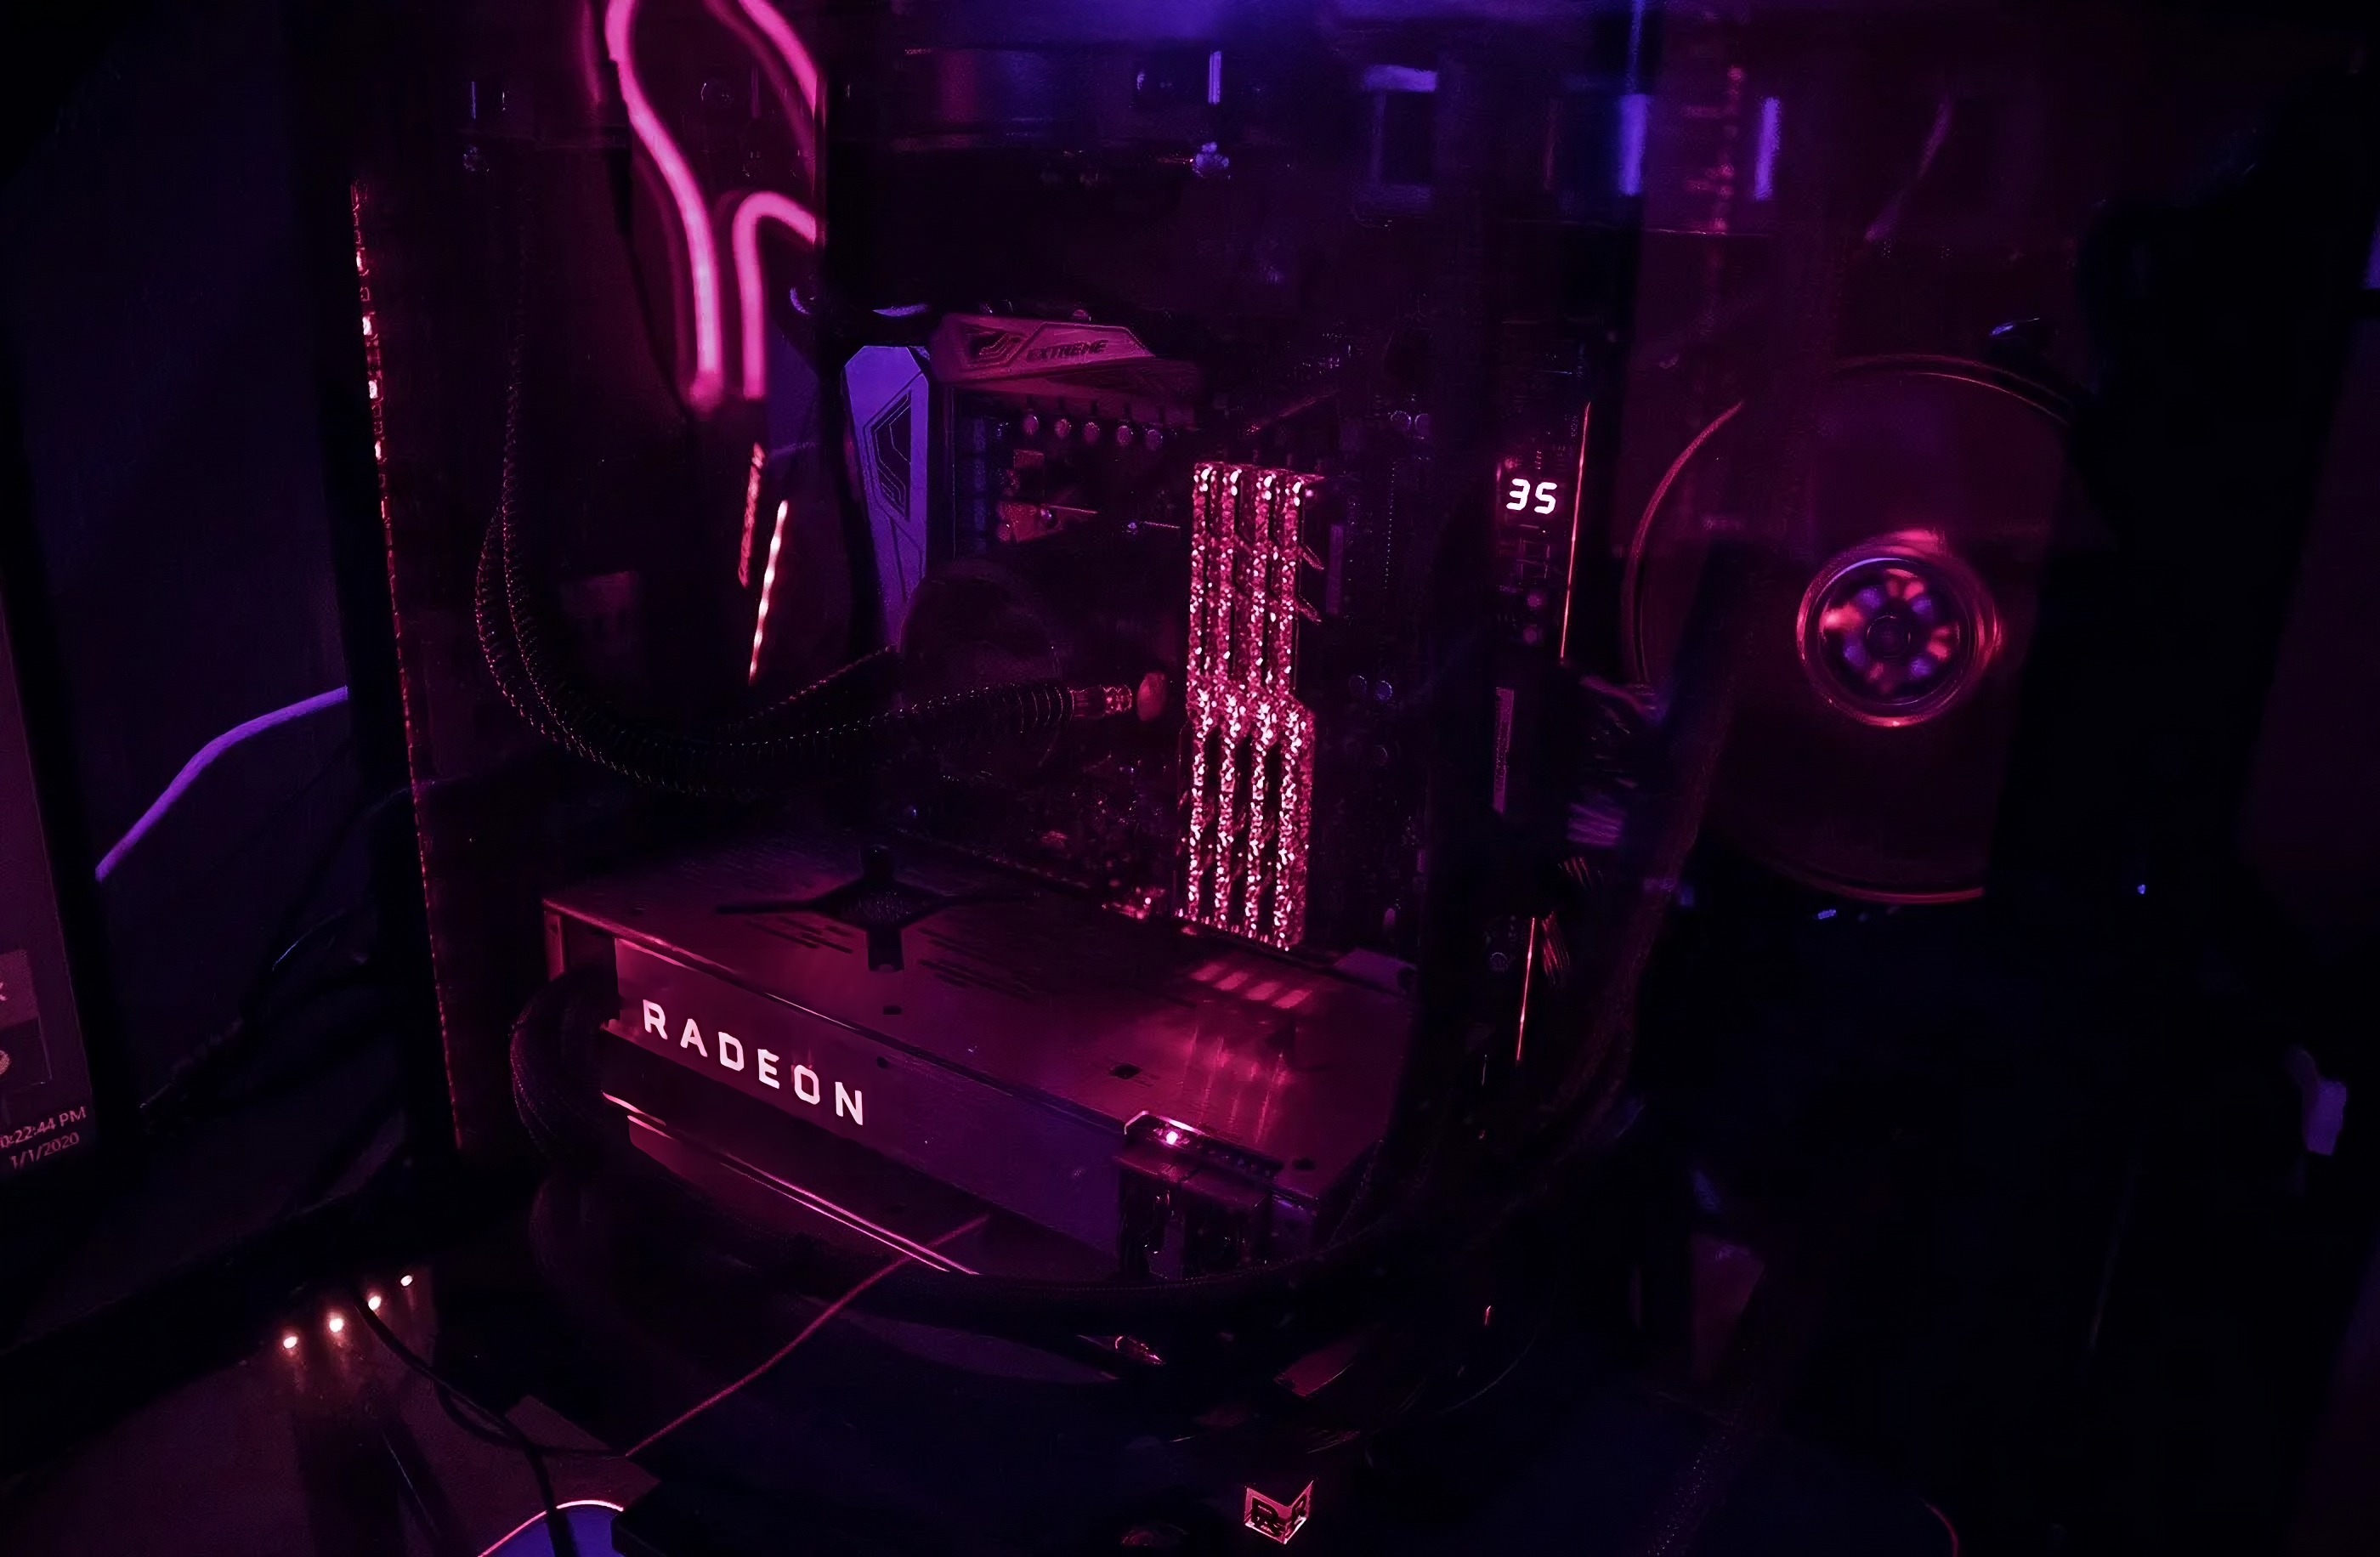
\includegraphics[width=\textwidth]{figures/001.png}}
    \caption[Google Trends data illustrating the ascent of Node.js and React Native.]{\textbf{Google Trends data illustrating the ascent of Node.js (in red) and React Native (in blue) from January 2004 to 2018.} The marked increase aligns with the period when JavaScript began to dominate server-side programming and mobile app development, demonstrating the language's versatility and the extensive ecosystem supported by NPM \citep{google_google_nodate}.}
    \label{fig:atwood-law}
  \end{figure}

  \section{WebGPU}
  \label{sec:webgpu}

  Before we can talk about WebGPU, let us first have a look at WebGL, and why it no longer has a future.

  \subsection{The Slow Death of WebGL}
  \label{subsec:the-slow-death-of-webgl}

  Do not get me wrong; WebGL is a fantastic piece of technology! It allows developers to create interactive 2D and 3D graphics which is impossible with standard JavaScript. Compared to, e.g. Flash, it allows developers to ship their content on the web without the need to install a plugin. The implementation of WebGL 1.0 and WebGL 2.0 is embedded in nearly all major browsers and even mobile phones.

  Since technologies usually do not vanish overnight, WebGL will definitely stay for many more years. Numerous applications and frameworks rely on WebGL, millions of people use them (Similarweb, n.d.), and hundreds of thousands of developers produce new software with WebGL each day (npm Inc., n.d.). This is entirely understandable because developers can create remarkable things with a low-level graphics API like WebGL. The most famous example is Google Maps — especially Google Earth (Shankland, 2011). Applications like that were unattainable until some years ago, and today we take it for granted to e.g. interact with 3D content on a website — even on mobile devices!

  WebGL gives developers the needed JavaScript binding to access the GPU. The WebGL API — especially shader programming in the Graphics Library Shader Language (GLSL) — is hard to use.

  Only a few developers — myself excluded — grasp the complexity of OpenGL and therefore also WebGL.

  That is why frameworks like Three.js, Babylon.js and Playcanvas came into existence. These frameworks are basically an abstraction on top of WebGL on top of OpenGL on top of the graphics cards to understand JavaScript code and render 2D/3D graphics in the browser. They are widely established and work great (Wappalyzer, n.d.). However, relying on a 10-year-old piece of technology has its downsides. Since the beginning in 2011, WebGL is based on OpenGL ES, a subset of the official OpenGL graphics API with various limitations like not using 3D textures, being limited to triangle meshes, and various others (The Khronos Group Inc., n.d.). WebGL is — from a high-level view — an API built on GPU technology’s understanding from around 15 years ago. Since then, many things have changed. One of the most notable changes is that modern GPUs usually work with shared memory access to perform parallel computing in a more performant fashion than before (Cabello and Wallez, 2019) — and that is where WebGPU comes into play.

  \subsection{Shared Memory}
  \label{subsec:shared-memory}

  To simply explain it with my beginner’s understanding: Shared memory is conceptually a place where each Arithmetic Logic Unit (ALU) can efficiently access logic of other ALUs instead of calculating it on its own (Wallez, 2020). I like to think of shared memory as a hashmap in dynamic programming that can optimise the space-time complexity in e.g. traversing through an input array with constant time operations to access data from the previous iterations instead of calculating them again on its own.

  Modern graphics card APIs such as Vulkan or Metal use concepts like shared memory — and many others — to optimise their performance. I like to think comparing OpenGL to e.g. Vulkan as comparing C to JavaScript: OpenGL — and therefore WebGL too — is slow because the other APIs are closer to the actual hardware and more or less platform-specific optimised as well (Hruska, 2015). OpenGL is not optimised for these new concepts. Many developers switched to Vulkan, Metal and co. because of these new concepts (like shared memory) and the benefits of a better performance. But why can’t we just create a new kind of OpenGL, which makes it possible to talk to all the modern graphics card APIs? Instead of porting an old native technology to the web, why can’t we just create a web API that provides some output that will be understood by the modern APIs (something similar to how WebAssembly works with the CPUs (Mozilla Foundation, 2021))? Well, that is precisely what the W3C intends to do with the new WebGPU browser standard.

  \subsection{A Group Effort}
  \label{subsec:a-group-effort}

  WebGPU is a group-effort between Apple, Google, Microsoft and many more and is currently being standardised by the W3C to replace WebGL (World Wide Web Consortium, n.d.). Compared to WebGL, WebGPU is not a port of an existing native graphics API to the web. It is based on concepts from e.g. Vulkan and aims to provide high performance on modern GPUs thanks to their optimised architecture (Wallez, 2018). It is intended to be able to write WebGPU specific JavaScript, which all the modern graphics card APIs will understand.

  Additionally, WebGPU is stateless and allows command reuse, meaning that sending instructions to the GPU is less expensive than with WebGL because it creates groups of instructions which will be used in advance (Cabello and Wallez, 2019). At runtime, it can switch between entire instruction groups with a single function call (thanks to shared memory). Shortly explained: The current implementation of WebGPU works a lot faster than WebGL — especially with a lot of 3D object instances in a complex scene.

  \subsection{The Limitation is The User}
  \label{subsec:the-limitation-is-the-user}

  All in all, WebGPU sounds almost too perfect. There is just one thing to consider: We ship the full source code to the client without knowing their hardware. What if the user visits a super-advanced science visualisation made with modern WebGPU technologies but has only an old onboard graphics card from 5 years ago? Well, their fault. It is the same as if a user still uses Internet Explorer in 2021; the typical compatibility misery. However, what if users still need even more elaborate 3D graphics and complex visualisations? What if the requirement exceeds the average consumer hardware? It sounds impossible, but a new type of technology allows developers to tackle this issue.

  \section{Pixel Streaming}
  \label{sec:pixel-streaming}

  Pixel streaming (or sometimes also called render streaming or remote rendering) makes it possible to stream the audio-visual output of a hosted cloud software to the client (Antunes, 2020). The client does not need expensive hardware — only a good internet connection.

  \subsection{How Pixel Streaming Works}
  \label{subsec:how-pixel-streaming-works}

  Basically, pixel streaming is about moving the heavy-lifting logic from the client to the server. It is the concept of developing software on dedicated hardware (with e.g. dedicated GPUs) and streaming the audio-visual output to the user. As a part of this, client-code (like JavaScript) will also be shipped to interact with the server’s software output in real-time (Epic Games Inc., n.d.). This makes pixel streaming from a developer’s perspective the less accessible technology compared to WebGL/WebGPU because it relies heavily on expensive hardware.

  Nevertheless, with pixel streaming, nearly everything seems possible! Developers can produce cutting-edge software which only runs on high-end graphics cards which users could never buy on their own — or even maintain.

  However, that is precisely the problem: scalability. A company/a developer needs to gain access to this high-end hardware. Of course, there are Infrastructure as a Service (IaaS) providers like Amazon Web Services (AWS) and Google Cloud Platform (GCP), but there is still a significant limitation: costs (Amazon.com Inc., n.d.). Even with AWS, GCP and co. in the backpack, running software on the required high-end hardware is a computationally expensive task that consumes a lot of energy. Yes, Google and co. seem to have a sheer endless amount of available computing power to make use of, but with the needs of a freely available pixel streaming application, one would push it to a costly limit.

  There are working proof of concepts like the Project Anywhere from NVIDIA, Microsoft and co. with streaming-optimised graphics cards (Woodard and Young, 2020) or even running products like Google Stadia (Patterson, 2020). However, the problem with overcoming the huge price factor is that a company cannot give away a pixel streaming application freely on the web; they would need a payment model for access. Otherwise, the company would possibly ruin themselves financially (imagine e.g. the cost of a DDoS attack on such a free to use application).

  \section{Hypothetical App: Virtual Offices}
  \label{sec:hypothetical-app-virtual-offices}

  Now that we know the technologies and some of the pros and cons let us imagine we want to build a 3D application in the near future. The application is called Hejm and aims to accommodate people from all over the world in a 3D virtual office. No matter what kind of business they run, Hejm provides them with the tools they will need for their remote-only office. Users can enter the office via virtual reality, augmented reality headsets or via a standard computer screen.

  \subsection{The Complexity of Pixel Streaming}
  \label{subsec:the-complexity-of-pixel-streaming}

  In a pixel streaming scenario, we would write the Hejm software to run on a cloud GPU instance (e.g. AWS EC2 GPU). We then create a client-side of the software that only provides the interaction JavaScript code to access the server-side logic via a real-time communication protocol. Something to be aware of is the problem that per accessing user, we would need to fire up an instance with the running software. It is possible to stream the output of one instance to multiple clients (and they can even all interact with it), but that is, yet again, another drawback. Multiplayer in this sense can — as of today — only be achieved with multiple instances (Epic Games Inc., n.d.), which pushes the costs too. For sure, we can modify our software so that it is optimised to run for more than one accessing user per instance. Nonetheless, there is still a vertical limit per GPU.

  Users should also be able to interact with each other in real-time and therefore require real-time server communication between instances. The instances also need a single source of truth for updates within the virtual office. There has to be a synchronisation module which updates all the different scenes on the other instances. However, this means that if e.g. many people move around or do things that are visible to all the other instances, simple functionalities can already be vast computational tasks and therefore costly. On top of this, there should be a chat, video and audio call features within the virtual office application which are expensive on their own.

  \subsection{A Hybrid Solution}
  \label{subsec:a-hybrid-solution}

  In a perfect hypothetical world, WebGPU would have >95\% browser compatibility and almost every conventional device supports the new standard, which would be very exciting times for Hejm! Hejm would have different product offerings, ranging from a free version, which runs only in the browser via WebGPU and an enterprise version which costs around 400\$/month per user. Companies that need the power of pixel streaming — e.g. simulating manufacturing CAD models or the like — would probably also be willing to pay extra for such a remote-first solution (they then could at least save on PC hardware and offices for their employees). I would even go further and display certain rooms in the virtual office only via pixel streaming and let the rest run via WebGPU in the browser — therefore being a hybrid solution.

  \section{Conclusion}
  \label{sec:conclusion}

  There is — as with many things — never a simple solution. But which technology should companies/developers use? I would say that it depends. Creating a high-end 3D software that can only run on high-end hardware with limited access and small user base: develop it with pixel streaming. If the application needs to be served to many thousands or even millions of users for free but does not require advanced features and visualisations: use WebGPU. If time allows it — and resources for research and development are available — I would encourage companies and developers to create a hybrid to satisfy both worlds’ requirements.

  I also personally think that a hybrid solution is an optimal answer in many software-related cases.

  I compare it with the discussion between Single-Page Applications (SPAs) and Multi-Page Applications (MPAs): First, the entire page was created on the server and sent as plain HTML/CSS/JS to the client. Then came Angular, React and co. and the UI logic layer shifted to the client; the server was only here to handle and serve the data. However, this solution was suboptimal: small websites used to send megabytes of JavaScript chunks just to display a simple UI (Tsarouva, 2019). This part of the web development industry is currently going into a hybrid phase as well: Server-Side Rendering (SSR) and Incremental Static Generation (ISG). Two different terms which deserve an article of their own; but in short: They solve the problem with pre-rendering the most critical software parts on the server and everything that needs to be asynchronous will be put together in the browser (Szczeciński, 2018).

  \section{Outlook}
  \label{sec:outlook}

  The entire topic about front vs back is an ongoing discussion in the web development/software industry. I do not think there will ever be a clear winner. It is exciting to see which of the two opponents in the graphics-world will be widely embraced — especially if pixel streaming is a thing to stay and how they want to overcome the high-price drawbacks. Moreover, maybe I am right with the hybrid solution, or perhaps an entirely new kind of technology enters the scene?



  % ! ==============================================
  % ! Start of the references and appendices content
  % ! ==============================================

  \pagebreak
  \bibliographystyle{../../templates/custom-apa}
  \bibliography{references/bibliography}

\end{sloppypar}
\end{document}
